\documentclass[11pt]{article}
\usepackage[margin=1in]{geometry}
\usepackage{graphicx}
\usepackage{booktabs}
\usepackage{hyperref}
\usepackage{tabularx}

\title{Do LLM Agents Know When They Are Done?\\Evaluating Specification Grounding in Tool-Using Agents}
\author{DoneBench Contributors}
\date{\today}

\begin{document}
\maketitle

\begin{abstract}
DoneBench evaluates whether tool-using agents can infer, formalize, stress-test, and act according to task-completion criteria before executing underspecified stateful tasks. Unlike benchmarks that hide success criteria in human or benchmark-provided graders, DoneBench makes completion-semantics construction itself the tested capability.
\end{abstract}

\section{Introduction}
Real tool-using agents often fail not because they cannot take actions, but because they do not know what would make the task complete. DoneBench isolates this capability as specification grounding: mapping a natural-language goal, visible state, tools, and policies into checkable completion semantics before execution.

Our narrow claim is not that DoneBench is the first agent benchmark, first rubric generator, or first verifier. The contribution is to evaluate whether the agent can write grader-like success semantics that it should later satisfy.

\section{Related Work}
Web and computer-use agent benchmarks emphasize realistic execution. WebArena provides self-hosted web applications across e-commerce, forums, software development, and content management, with 812 end-to-end web tasks scored by functional correctness \href{https://arxiv.org/abs/2307.13854}{[WebArena]}. OSWorld moves this style to real desktop environments, with 369 tasks spanning web apps, desktop apps, file I/O, and multi-application workflows, each paired with setup and execution-based evaluation scripts \href{https://arxiv.org/abs/2404.07972}{[OSWorld]}. WorkArena and WorkArena++ focus on enterprise knowledge work in ServiceNow: WorkArena introduces 33 browser-based tasks, while WorkArena++ expands to 682 compositional tasks and ground-truth traces for planning and reasoning analysis \href{https://arxiv.org/abs/2403.07718}{[WorkArena]}, \href{https://arxiv.org/abs/2407.05291}{[WorkArena++]}. $\tau$-bench evaluates multi-turn tool-agent-user conversations in airline and retail domains using policy guidelines, API tools, final database-state comparison, and pass$^k$ reliability \href{https://arxiv.org/abs/2406.12045}{[$\tau$-bench]}. Across these benchmarks, the dominant validation pattern is executable or functional grading rather than mandatory double annotation of every task; DoneBench follows that tradition with reference replay, state-based grading, and task-quality audit, while treating human calibration as an optional strengthening layer.

These benchmarks share DoneBench's concern with state, tools, policies, and reproducible outcome grading, but they mostly keep the completion semantics inside the benchmark grader. DoneBench instead asks the agent to state those semantics before execution, scores atom-level agreement with hidden gold criteria, stress-tests the produced verifier on near-miss states, and then checks whether execution violates the agent's own criteria. This makes the tested object different from final task success: the central capability is knowing what would count as done before acting.

Evaluation frameworks and utility-assessment systems are adjacent but not substitutes. AgentEval automatically proposes task-specific utility criteria and applies them to LLM-powered applications \href{https://arxiv.org/abs/2402.09015}{[AgentEval]}, while DeepEval provides unit-test-like metrics, LLM-as-judge metrics, tracing, synthetic datasets, and CI workflows for LLM applications \href{https://deepeval.com/docs/introduction}{[DeepEval]}. These systems help practitioners define and run evaluations, but they do not package a stateful workflow benchmark where criterion construction itself is the model output under test.

Specification and verifier benchmarks provide another close boundary. CodeSpecBench evaluates executable behavioral specification generation for code, including function-level and repository-level Python specifications with correctness and completeness checks \href{https://arxiv.org/abs/2604.12268}{[CodeSpecBench]}. RESTestBench evaluates LLM-generated REST API tests from natural-language requirements using three REST services, precise and vague requirement variants, and requirement-based mutation testing \href{https://arxiv.org/abs/2604.25862}{[RESTestBench]}. VerifyLLM verifies robotic task plans before execution by translating natural-language instructions into Linear Temporal Logic and analyzing action sequences \href{https://arxiv.org/abs/2507.05118}{[VerifyLLM]}. DoneBench borrows the insight that executable specifications and adversarial invalid cases are essential, but shifts the domain from program or robot-plan verification to everyday tool-using workflow agents and ties specification grounding to downstream execution and self-violation metrics.

\section{DoneBench}
Each task contains a user goal, visible tool environment, initial state, policies, gold criterion atoms, a DoneSpec verifier, near-miss mutated final states, and a reference solution trace.

DoneBench separates reference validation from agent execution. The reference trace is used to validate that the gold DoneSpec accepts at least one intended completion and rejects near misses. Agent trials instead use a tool-plan executor: the model emits structured tool calls, the environment checks tool availability and preconditions, records confirmations and side effects, mutates the state through domain tool semantics, and then grades the resulting state and trace. This prevents the execution score from being a direct copy of the benchmark-provided final state.

\begin{figure}[h]
\centering
\fbox{\parbox{0.86\linewidth}{Task input $\rightarrow$ pre-execution spec $\rightarrow$ near-miss verifier test $\rightarrow$ structured tool plan $\rightarrow$ environment execution $\rightarrow$ gold and own-spec grading.}}
\caption{DoneBench pipeline.}
\end{figure}

\begin{figure}[h]
\centering
\fbox{\parbox{0.86\linewidth}{Domains: calendar, email, spreadsheet/database, CRM workflow, and file/document operations. Each item has state, policies, side-effect constraints, temporal constraints, and mutations.}}
\caption{Domain/task construction schema.}
\end{figure}

\section{Metrics}
Completion Criterion F1 measures atom-level agreement between predicted and gold hard criteria. Overconstraint rate counts unmatched predicted hard atoms; underspecification rate counts unmatched gold hard atoms.

Near-miss detection and verifier robustness evaluate whether the agent's own DoneSpec rejects superficially successful but invalid states. Spec-execution alignment measures whether the final state and trace violate the agent's own hard criteria.

\begin{figure}[h]
\centering
\fbox{\parbox{0.86\linewidth}{Good spec/good execution; good spec/bad execution; bad spec/good execution; bad spec/bad execution.}}
\caption{Four-quadrant spec/execution taxonomy.}
\end{figure}

\begin{table}[h]
\centering
\begin{tabular}{ll}
\toprule
Metric & Purpose \\
\midrule
CC-F1 & Pre-execution completion semantics \\
Near-miss detection & Rejection of invalid final states \\
Task success & Gold deterministic final-state grading \\
Self-violation rate & Execution against own criteria \\
\bottomrule
\end{tabular}
\caption{Metrics.}
\end{table}

\section{Experimental Setup}
The local smoke configuration runs without paid APIs using deterministic MockLLM-compatible agents. API-backed adapters are configured but treated as optional until credentials and budget are available.

Experiments measure criterion inference, spec-first execution, own-spec violations, verifier robustness, and model scaling. Statistical reporting uses task-level bootstrap confidence intervals and domain/difficulty stratification.

\subsection{Planned Evaluation Matrix}

The MVP paper artifact separates deterministic smoke tests from API-backed paper runs. Smoke tests are intended for every checkout and continuous integration. API-backed runs are intended for the final paper tables once credentials, budget, and model identifiers are fixed.

\begin{table}[h]
\centering
\begin{tabular}{llll}
\toprule
Suite & Split & Agents & Models \\
\midrule
Smoke & dev & Heuristic, Spec-first & Mock \\
Full API & test & Direct, Plan-first, Spec-first, Oracle-spec & GPT-, Claude-, Gemini-, OpenRouter-compatible, Ollama \\
\bottomrule
\end{tabular}
\caption{Experiment suites mirrored by \texttt{configs/experiments.yaml}.}
\end{table}

\subsection{Baselines and Ablations}

Direct runs execute with only implicit completion checks. Plan-first elicits action order and dependencies before acting. Spec-first explicitly elicits completion criteria and a DoneSpec before acting. Oracle-spec receives the gold verifier and estimates the execution gap after specification ambiguity is removed. Mock and oracle-backed paths are treated as harness sanity checks; paper claims should use live-model rows and separately report token-matched controls.

\begin{table}[h]
\centering
\begin{tabular}{lll}
\toprule
Ablation & Purpose & Paper status \\
\midrule
Direct vs. Plan-first & Separate planning from completion semantics & Placeholder \\
Plan-first vs. Spec-first & Test the value of explicit done criteria & Placeholder \\
Spec-first vs. Oracle-spec & Estimate residual execution failure & Placeholder \\
Near-miss mutation families & Stress-test verifier robustness & Placeholder \\
Token-matched prompting & Control for prompt length & Future paper run \\
Free-form criterion normalization & Test DSL sensitivity & Future paper run \\
\bottomrule
\end{tabular}
\caption{Ablation checklist for paper-ready experiments.}
\end{table}

\subsection{API Run Protocol}

Hosted-model results should report provider, model identifier, access date, decoding parameters, retries, and trial count. Runs should be launched only after the relevant environment variable is set in the active shell. Missing credentials are skipped when \texttt{skip\_missing\_credentials: true}, which prevents smoke reproduction from failing on machines without API access.

\section{Results}
Smoke results are generated by \texttt{make smoke}. The MVP reports local heuristic and spec-first baselines on the development split, with figures saved under \texttt{paper/figures/}.

\begin{table}[h]
\centering
\begin{tabular}{llllll}
\toprule
Suite & Agent & Model & CC-F1 & Task success & Near-miss detection \\
\midrule
Smoke & Heuristic & Mock & see \texttt{paper/tables/main\_results.csv} & see CSV & see CSV \\
Smoke & Spec-first & Mock & see \texttt{paper/tables/main\_results.csv} & see CSV & see CSV \\
Full API & Direct & TBD & Placeholder & Placeholder & Placeholder \\
Full API & Plan-first & TBD & Placeholder & Placeholder & Placeholder \\
Full API & Spec-first & TBD & Placeholder & Placeholder & Placeholder \\
Full API & Oracle-spec & TBD & Placeholder & Placeholder & Placeholder \\
\bottomrule
\end{tabular}
\caption{Main results table template. Replace placeholders with audited API-backed aggregates before submission.}
\end{table}

\begin{table}[h]
\centering
\begin{tabular}{lllll}
\toprule
Domain & Agent & CC-F1 & Task success & Near-miss detection \\
\midrule
Calendar & TBD & Placeholder & Placeholder & Placeholder \\
Email & TBD & Placeholder & Placeholder & Placeholder \\
Sheet/database & TBD & Placeholder & Placeholder & Placeholder \\
CRM/workflow & TBD & Placeholder & Placeholder & Placeholder \\
File/document & TBD & Placeholder & Placeholder & Placeholder \\
\bottomrule
\end{tabular}
\caption{Domain-stratified results template. The smoke aggregate is exported to \texttt{results/by\_domain.csv}.}
\end{table}

\begin{figure}[h]
\centering
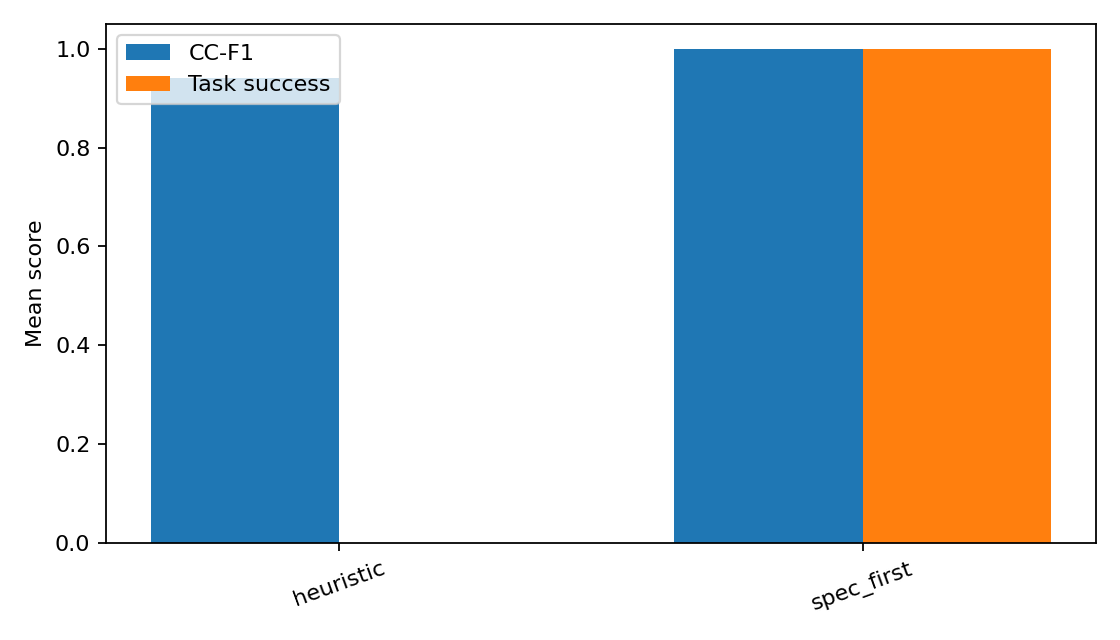
\includegraphics[width=0.8\linewidth]{figures/main_results_by_agent.png}
\caption{Results by agent.}
\end{figure}

\begin{figure}[h]
\centering
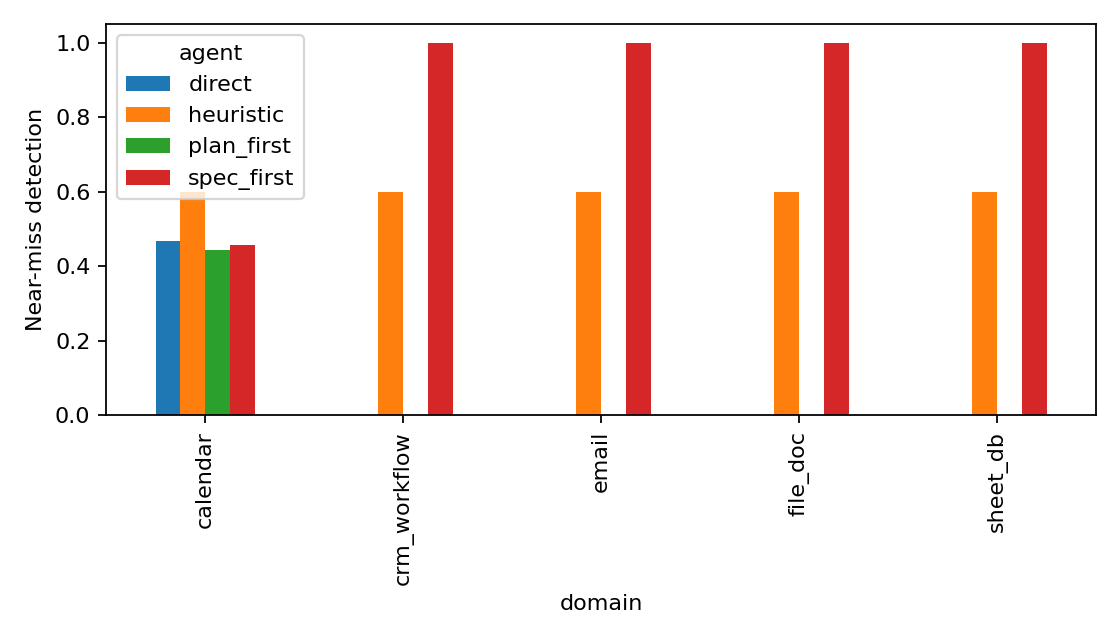
\includegraphics[width=0.8\linewidth]{figures/near_miss_by_domain.png}
\caption{Near-miss mutation examples and detection by domain.}
\end{figure}

\section{Analysis}

\subsection{Specification-to-Execution Diagnostic Protocol}

DoneBench is intended as a diagnostic benchmark, not as a new agent algorithm. Its central analysis decomposes task completion into four observable gates. First, criterion inference asks whether the agent recovers the hard completion conditions from the user goal, visible tools, state, and policies. Second, executable encoding asks whether those criteria become a runnable DoneSpec verifier. Third, near-miss robustness asks whether the verifier rejects plausible but invalid final states. Fourth, own-spec compliance asks whether the agent's tool execution satisfies the hard criteria it stated for itself.

This protocol exposes failures hidden by task success alone. The four-quadrant table in \texttt{paper/tables/four\_quadrants\_full\_toolplan.csv} separates good-spec/good-execution, good-spec/bad-execution, bad-spec/good-execution, and bad-spec/bad-execution cases by model, agent, and domain. The current DeepSeek tool-plan full run is dominated by bad-spec/bad-execution, with good-spec/bad-execution as the important secondary mass. That pattern supports a narrow claim: agents can improve measured completion-criteria quality while still failing to operationalize those criteria during tool use.

Self-violation diagnostics further show that explicit criteria are not enough. \texttt{paper/tables/self\_violation\_by\_signature\_full\_toolplan.csv} groups own-spec failures by observable trace signatures such as missing confirmation or state-only final-state mismatch. These signatures are not human-validated semantic labels; they are trace-grounded evidence that an agent can write a verifier and still produce a final state or action trace that fails it.

Near-miss diagnostics link verifier robustness to execution outcomes. \texttt{paper/tables/near\_miss\_success\_full\_toolplan.csv} reports near-miss detection and task success by failure family. This makes the benchmark different from a single pass/fail workflow score: a model may reject some non-completions, accept others, and still fail the final task.

\begin{table}[tbp]
\centering
\small
\begin{tabularx}{\linewidth}{lX}
\toprule
Diagnostic gate & Paper-facing artifact \\
\midrule
Criterion inference & \texttt{paper/tables/main\_results\_full\_toolplan.csv} \\
Executable verifier encoding & \texttt{paper/tables/main\_results\_full\_toolplan.csv} \\
Near-miss robustness & \texttt{paper/tables/near\_miss\_success\_full\_toolplan.csv} \\
Own-spec compliance & \texttt{paper/tables/self\_violation\_by\_signature\_full\_toolplan.csv} \\
Spec/execution disagreement & \texttt{paper/tables/four\_quadrants\_full\_toolplan.csv} \\
\bottomrule
\end{tabularx}
\caption{Specification-to-execution diagnostic protocol. These artifacts reorganize existing DeepSeek tool-plan full-run evidence and should not be read as a new performance-improving method.}
\end{table}

\subsection{Boundaries}

The main 18,000-trial DeepSeek run predates the full-corpus reference-artifact repair. We therefore use it as the largest completed diagnostic run and report repaired-corpus strict validation, oracle reference replay, token-matched controls, and a 600-trial repaired-corpus confirmation slice separately. The confirmation slice is not a replacement for the full-run table: it covers 100 repaired tasks with DeepSeek V4 Flash/Pro and has one quarantined model-agent cell because \texttt{deepseek\_v4\_pro} with \texttt{spec\_first} exceeded the parse fallback threshold. Cross-family suites are configured for DeepSeek, Qwen, GLM, and Kimi, but they remain pending until at least three provider families produce complete rows. Human calibration is useful but optional; model- or agent-assisted packets must not be described as completed human annotation.

\section{Limitations}
The current dataset is controlled and generator-assisted rather than a real GUI or SaaS environment. This is a deliberate tradeoff for isolating completion-semantics grounding, but it means DoneBench should be positioned as complementary to WebArena, OSWorld, WorkArena, and tau-bench rather than more realistic than them. We therefore report lexical and structural diversity audits, family-leakage tables, a task-construction datasheet, executable reference replay, near-miss rejection checks, and model-assisted task-quality audit. Human calibration remains a limitation: it would strengthen semantic-validity claims, but the current paper gate relies on executable validation and structured/model-assisted audit rather than double annotation. Criterion matching is deterministic for atom outputs, while free-form paraphrase calibration remains a limitation. API-backed results may drift as hosted models change.

\section{Ethics and Release Considerations}
The benchmark avoids private data and paid services by default. Release should include dataset documentation, task-audit procedures, and clear caveats about synthetic workflow coverage.

\section{Conclusion}
DoneBench makes a falsifiable question measurable: whether agents know what task completion requires before they act, and whether they can operationalize those criteria during execution.


\appendix
\section{Reproducibility and Artifact Checklist}

DoneBench is designed to be reproducible without paid model access for smoke testing, while allowing paper experiments to be rerun with hosted or local LLM providers. The artifact should be released with the task data, deterministic DoneSpec graders, near-miss mutations, run configuration, raw JSONL traces, aggregate CSV files, and generated figures.

\begin{table}[h]
\centering
\begin{tabular}{lp{0.62\linewidth}}
\toprule
Artifact item & Expected location or command \\
\midrule
Task data and splits & \texttt{data/tasks} with dev/test metadata \\
Experiment config & \texttt{configs/experiments.yaml} \\
Smoke run & \texttt{make smoke} \\
Raw traces & \texttt{results/*.jsonl} \\
Aggregates & \texttt{results/by\_agent.csv}, \texttt{results/by\_domain.csv}, \texttt{results/taxonomy.csv} \\
Paper figures & \texttt{paper/figures/} generated by \texttt{donebench make-figures} \\
Paper tables & \texttt{paper/tables/} templates or exported CSVs \\
\bottomrule
\end{tabular}
\caption{Paper artifact checklist.}
\end{table}

\paragraph{API-backed experiments.}
Live model runs require installing the optional LLM dependency group and setting one or more provider credentials in the shell that launches the benchmark:

\begin{verbatim}
python -m pip install -e ".[dev,llm]"
$env:OPENAI_API_KEY="sk-..."
$env:ANTHROPIC_API_KEY="..."
$env:GEMINI_API_KEY="..."
$env:OPENROUTER_API_KEY="..."
$env:OLLAMA_BASE_URL="http://localhost:11434"
donebench run --config configs/experiments.yaml --split test --agent spec_first --model gpt_compatible
donebench aggregate results/
donebench make-figures results/ paper/figures/
\end{verbatim}

Only the relevant provider variable is needed for a given model adapter. Credentials must not be committed; paper artifacts should report model identifiers, provider date, decoding settings, trial count, and whether missing providers were skipped by \texttt{skip\_missing\_credentials}.

\paragraph{Submission checklist.}
Before submission, regenerate all tables from raw traces, record package versions and hosted model identifiers, run each planned API condition for the configured trial count, and freeze the exact commit used for the paper artifact.


\bibliographystyle{plain}
\bibliography{references}
\end{document}
